%!TEX encoding = UTF-8 Unicode
%!TEX program = xelatex

\documentclass[bachelor]{ustcthesis}
% bachelor|master|doctor
\usepackage{ustcextra}
\usepackage{listings}
\lstset{language=C++}
\graphicspath{{figures/}}
%\bibliographystyle{ustcauthoryear}
\bibliographystyle{ustcnumerical}
\title{利用ClickNP实现RDMA协议及其性能测试}
\author{李弈帅}
\major{计算机科学与技术}
\advisor{谭焜\ 研究员\\&孙广中\ 副教授}
\submitdate{二〇一六年六月}
%\secrettext{机密\quad 小于等于20年}   % 内部|秘密|机密,注释本行则不保密
\depart{零系}

\entitle{Implementation and evaluation of RDMA protocol with ClickNP}
\enauthor{Yishuai Li}
\enmajor{Computer Science and Technology}
\enadvisor{Rsr. Kun Tan\\&A. Prof. Guangzhong Sun}
\ensubmitdate{June, 2016}
%\ensecrettext{Confidential\quad Less than or equal to 20 years}  % Internal|Secret|Confidential

\begin{document}

\maketitle

%
% 本科论文:
%   frontmatter: 致谢、目录、中文摘要、英文摘要
%   mainmatter: 正文章节、参考文献
%   appendix: 附录
%
% 硕博论文:
%   frontmatter: 中文摘要、英文摘要、目录、符号说明
%   mainmatter: 正文、参考文献
%   appendix: 附录
%   backmatter: 致谢、发表论文
%
\frontmatter
\begin{acknowledgements}

在研究学习期间,我有幸得到了我的导师,
微软亚洲研究院谭\raisebox{-0.1em}{
\includegraphics[height=0.9em,keepaspectratio=true]{kun}}研究员的教导。
他深厚的学术功底,严谨的工作态度和敏锐的科学洞察力使我受益良多。
我谨在此衷心感谢他给予我的悉心教导和热情帮助。

在微软实习期间,无线与网络研究组的李博杰、陆元伟、罗人千三位同事给予了我莫大的帮助,
使我快速适应了新的工作氛围及研究课题,在我遇到困难的时候提供了经验与思路。谨一并表示感谢。

感谢科大的陈意云、冯新宇、孙广中、张昱四位老师对我出国申请的大力帮助,
他们的支持是我继续努力攻读博士学位的动力。

感谢我的班主任李娜颖老师四年以来在学习、工作、生活等方面对我的教导,
帮助我在科大避开许多弯路迅速成长。

感谢我的家人对我持之以恒的关爱与支持。我的家人不仅抚育我长大成人,
而且培养了我对科学的兴趣,给了我自主选择未来发展道路的权利,
鼓励我探索外面的世界,对我从中学到大学的成长产生了深刻影响。

另外,感谢我的女朋友。在过去的21年间,她不曾出现在我的生活中,使我专注于学术,心无旁骛。

\bigskip
\rightline\today

\end{acknowledgements}


%  move main matter here because of indexing.
\mainmatter
\tableofcontents
\listoffigures
%\listoftables
%\listofalgorithms  % 算法索引,如不需要,可直接注释掉本行
\begin{abstract}
  灵活的软件定义网络功能对于多客户的数据中心至关重要。
  现有的基于通用服务器的软件处理网络包面临高延迟、低吞吐率等问题,
  而场效可编程门阵列(field-programmable gate array, FPGA)
  具有高性能、高并行、低能耗等特点,更符合软件定义网络的计算需求。
  本文针对五个数据中心网络应用,使用FPGA平台进行性能优化及评测,
  以提升其带宽并降低延迟。

  \keywords{数据中心网络\zhspace{} 软件定义网络\zhspace{} 场效可编程门阵列}
\end{abstract}

\begin{enabstract}
  Highly flexible software network functions are critical components to multi-tenant data centers.
  However, commodity servers are faced with high latency and limited capacity when processing software packets.
  In comarison, field-programmable gate arrays show advantage in performance, parallelizability and power efficiency,
  which fits the need of software-defined networking.
  This article is to optimize and evaluate five data center network applications with the FPGA platform.
\enkeywords{data center network, software-defined networking, FPGA}
\end{enabstract}

% \input{chapters/notation}

\chapter{绪论}
\section{数据中心网络}
现代数据中心在共享的设备资源基础上,为多个用户提供不同的服务。
为保障数据安全以及用户的独立性,数据中心向每个用户展现的是虚拟化的网络环境。
这就需要数据中心的管理者部署灵活的网络功能来实现这一要求。

由于硬件网络设备普遍灵活性受限,几乎所有的云服务商都用软件来实现其网络功能,
例如:微软、亚马逊、VMWare等\cite{azure, 179731}。但软件实现网络功能的性能天然存在两个问题:

其一,吞吐率受限。现有的软件定义网络功能通常需要使用两个以上核才能达到10Gbps带宽
\cite{Martins:2014:CAN:2616448.2616491,180672},
而最新的网络设备带宽已达到40\textasciitilde 100Gbps\cite{edr}。
尽管增加单服务器的核数能够提升部分性能,但与此同时成本也会大幅提升。
一方面是设备开销提高,另一方面则是能耗显著增加。

其二,延迟高且不稳定。现有软件定义网络的处理延迟从几十微秒到毫秒量级不等
\cite{Gandhi:2014:DCS:2619239.2626317, Martins:2014:CAN:2616448.2616491, Gandhi:2014:DCS:2619239.2626317}。
无法满足证券交易等对低延迟要求严苛的应用需求。

在图形处理器(graphics processing unit, GPU)\cite{Han:2010:PGS:1851275.1851207}、
专用网络处理器\cite{cavium, netronome}和FPGA\cite{sigcomm2015keynote, Naous:2008:NRR:1397718.1397720}
上均有相关的工作旨在保障灵活性的基础上克服软件处理网络包的上述限制。
相比于GPU而言,FPGA能耗更低\cite{5681761, 5572788};相比于专用网络处理器,FPGA可通过硬件逻辑实现更多服务所需的功能。
更重要的是,将FPGA部署在大规模数据中心的成本更低\cite{sigcomm2015keynote,6853195}。

在数据中心中利用FPGA加速软件网络功能从预期上能够达到较好的性能,
但实践中面临的主要问题是编程方面困难。传统的FPGA逻辑是通过Verilog、VHDL等硬件描述语言编写,
这些语言所展现的是门、寄存器、多路选择器、时钟等非常底层的器件。
这样虽然方便手工优化逻辑,但也导致编程复杂度高、开发效率低下、调试方面等问题。
这些困难导致多年来很多人远离FPGA编程\cite{Bacon:2013:FPM:2436256.2436271}。

本文借助微软亚洲研究院无线与网络研究组最新开发的ClickNP平台\cite{clicknp}进行FPGA编程,
针对数据中心网络场景优化了包生成器及抓包器、OpenFlow防火墙、IPSec网关、L4负载均衡、pFabric流调度器等应用,
并对其性能进行评测。

\section{场效可编程门阵列体系结构}
场效可编程门阵列(FPGA)由大量逻辑门组成。其基本编程单元为逻辑块,由查找表和寄存器组成。
其中查找表可编程为任何组合逻辑计算,寄存器可以存储状态。
FPGA还包含存储数据的块随机访问存储器(block random access memory)、
处理复杂算术运算的数字信号处理单元(digital signal processing)。
FPGA通过PCIe子板与主机相连,其中子板包含数G字节的动态随机访问存储器(dynamic random access memory)
以及10G/40G以太网端口等其他通信界面。

相比于CPU和GPU而言,FPGA的时钟频率较低、访存带宽较小。
典型的FPGA时钟频率在200MHz左右,相比于时钟频率2\textasciitilde 3GHz的CPU低一个多数量级。
FPGA到单个块存储器和外部的动态存储器的带宽约为2\textasciitilde 4GBps,
而英特尔至强处理器的访存带宽约为40GBps,GPU的带宽则高达100GBps。

但相比于被有限核数限制并行数的CPU和GPU而言,FPGA的可并行化程度较高。
现代的FPGA可以集成数百万个逻辑块、数百Kbit寄存器、数十Mbit块存储器以及数千个数字信号处理单元。
理论上,所有这些器件均可并行地工作。因此数千个“核”在同一个FPGA芯片中并行工作是有可能的。
尽管单个块存储器的带宽有限,但同时访问数千个块存储器可使带宽达到TBps量级。
因此,为了在FPGA平台上实现高性能,必须充分利用其并行化的能力。

传统的FPGA编程使用Verilog、VHDL等硬件描述语言实现。这些语言关注底层细节,难于学习,编程复杂。

为了减轻编程负担,工业界与学术界均有开发高级编程工具,将以C语言为主的高级语言编写的程序转化为硬件程序。
其中包括微软亚洲研究院无线与网络研究组开发的ClickNP编程平台\cite{clicknp}。

\section{RoCEv2远程直接数据存取协议}
\subsection{直接数据存取}
直接数据存取 (direct memory access, DMA) 是现代计算机系统中常见的访存方式,
这种方式使外围设备可以不经CPU而直接访问存储器。

在非DMA访存模式下,CPU采用可编程输入输出方式与外围设备进行数据交互。
在等待设备完成读写操作期间,CPU无法处理其他任务,这一停等浪费大量计算资源。

在DMA访存模式下,CPU将数据传输初始化,在随后的数据传输过程中处理其他任务。
在数据传输结束时,会从DMA控制器收到表明操作完成的中断。
这一特性既适用于数据传输率远高于CPU处理能力的情况,
也适用于需要CPU利用等待时间处理更重要任务的情况。

\subsection{远程直接数据存取}
远程直接数据存取 (remote direct memory access, RDMA) 是不经过任何一台设备上操作系统的设备间访存方式。

RDMA设备接收到特定的数据包之后不再交由操作系统处理,而直接根据其请求访问本地存储器并进行反馈。
而CPU只负责初始化和结束RDMA设备,在数据传输过程中不会收到中断请求。

\subsection{RoCE协议}
基于融合以太网络的RDMA (RDMA over Converged Ethernet, RoCE) 协议允许设备间通过以太网络进行远程直接内存访问。
该协议由两个版本,分别称为RoCEv1和RoCEv2。其中RoCEv1将以太网协议作为其链路层该协议,
因而允许在同一个以太网广播域下的任意两台主机间进行通信\cite{a16}。
RoCEv2则基于用户数据报协议 (user datagram protocol, UDP),因而可以经过路由\cite{a17, considerations, storage}。

\begin{figure}[htbp]
\centering
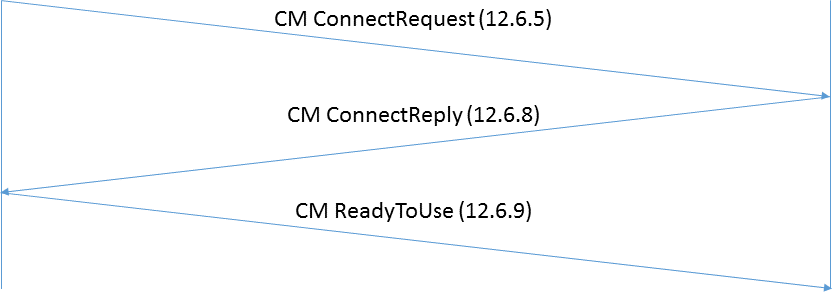
\includegraphics[width=4in]{rocereq}
\caption{建立RoCE连接} \label{fig:rocereq}
\end{figure}

\begin{figure}[htbp]
\centering
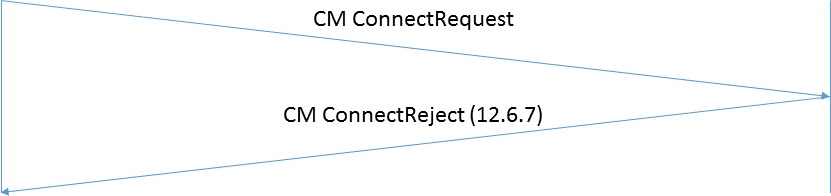
\includegraphics[width=4in]{rocerej}
\caption{建立RoCE连接被拒绝} \label{fig:rocerej}
\end{figure}

\begin{figure}[htbp]
\centering
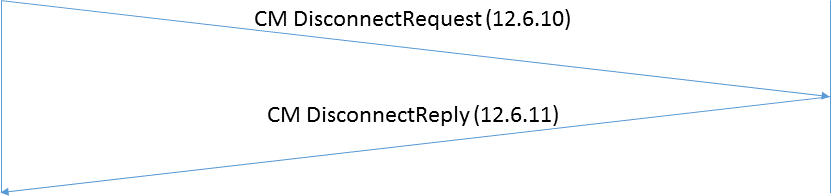
\includegraphics[width=4in]{rocedreq}
\caption{断开RoCE连接} \label{fig:rocedreq}
\end{figure}

\begin{figure}[htbp]
\centering
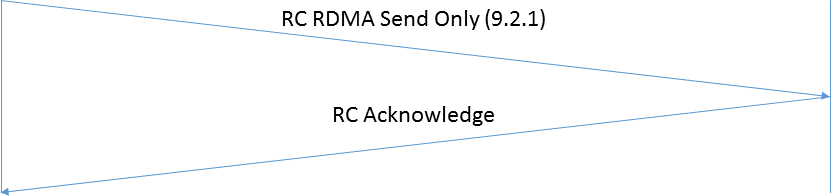
\includegraphics[width=4in]{rocewriteonly}
\caption{单RoCE包写操作} \label{fig:rocewriteonly}
\note{在数据载荷不多于1024字节时的写请求只包含单包,数据发送请求的工作过程与之类似。}
\end{figure}

\begin{figure}[htbp]
\centering
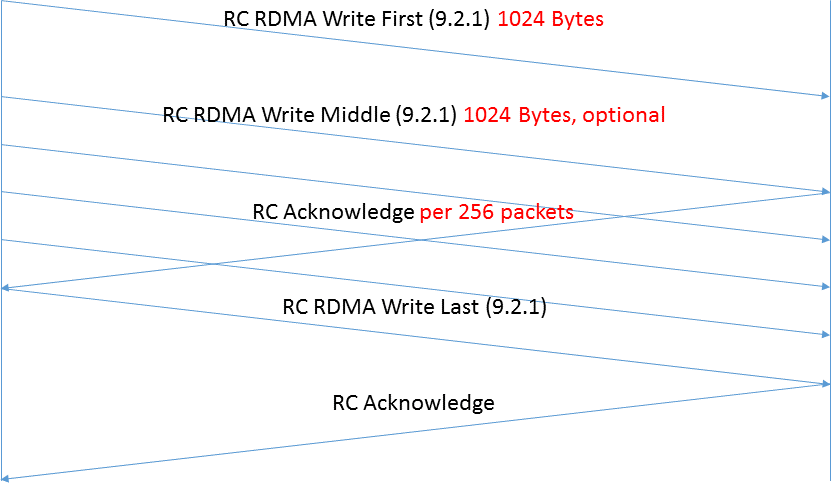
\includegraphics[width=4in]{rocewritemany}
\caption{多RoCE包写操作} \label{fig:rocewritemany}
\note{对于超过1024字节的数据载荷,先后发送Write First、Write Middle (如有)、Write Last三种包。
自Write First起,接收端每收到256个包反馈一个确认包,也对最后一个包进行反馈,
数据发送请求的工作过程与之类似。}
\end{figure}

\begin{figure}[htbp]
\centering
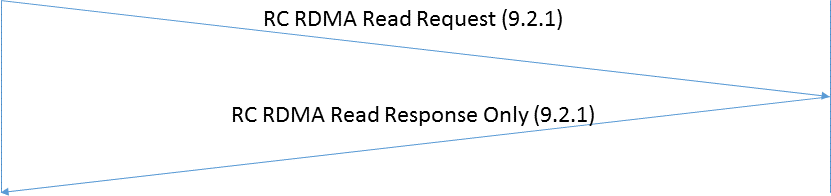
\includegraphics[width=4in]{rocereadonly}
\caption{单RoCE包读操作} \label{fig:rocereadonly}
\note{在数据载荷不多于1024字节时读响应至包含单包}
\end{figure}

\begin{figure}[htbp]
\centering
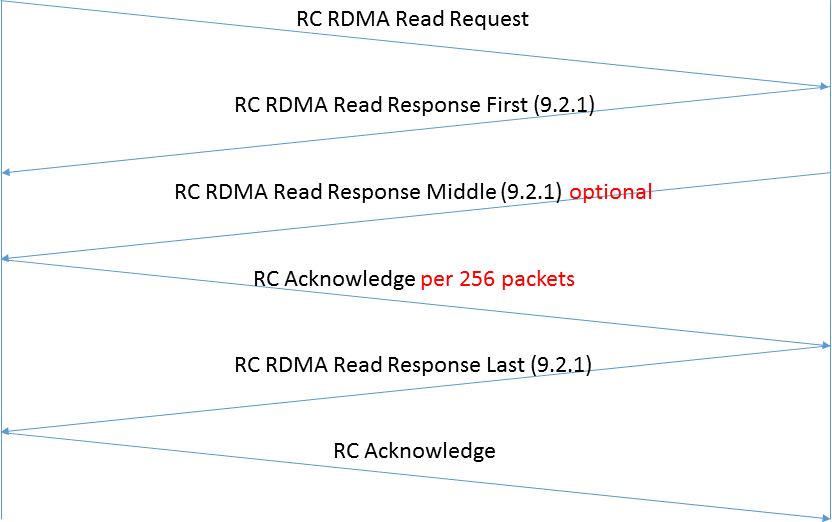
\includegraphics[width=4in]{rocereadmany}
\caption{多RoCE包读操作} \label{fig:rocereadmany}
\note{对于超过1024字节的数据载荷,先后发送Read Response First、Read Response Middle (如有)、
Read Response Last三种包。自Read Response First起,接收端没收到256个包反馈一个确认包,
也对最后一个包进行反馈。}
\end{figure}

用户可通过RoCE协议发起读数据、写数据、发送数据三种请求。
其工作过程如图~\ref{fig:rocereq}、图~\ref{fig:rocerej}、图~\ref{fig:rocedreq}、
图~\ref{fig:rocewriteonly}、图~\ref{fig:rocewritemany}、图~\ref{fig:rocereadonly}所示。

面对网络中可能出现的丢包情况,RoCE协议具有与TCP/IP类似的重传策略:
对每个消息赋予一个包序列号。如果接收端收到的包序列号不连续,则反馈缺失消息,
并提供缺失的第一个包序列号。发送端从该序列号对应的包开始重传,如图~\ref{fig:rocewritenak} 所示。
\begin{figure}[htbp]
\centering
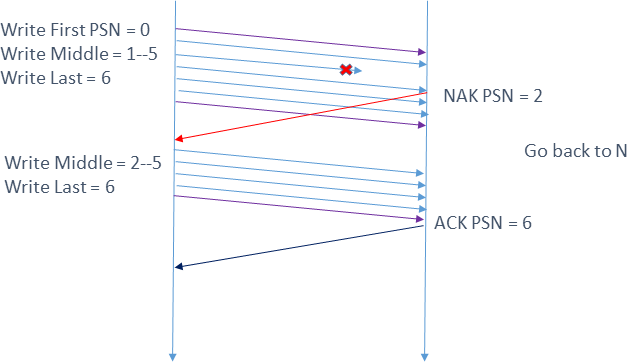
\includegraphics[width=4in]{rocewritenak}
\caption{RoCE重传策略} \label{fig:rocewritenak}
\end{figure}


\chapter{背景介绍:ClickNP编程工具}
ClickNP是微软亚洲研究院开发的FPGA编程工具\cite{clicknp}。
\section{系统架构}
ClickNP基于Catapult Shell体系结构\cite{6853195}搭建。该体系结构包含PCIe、直接内存访问(direct memory access, DMA)、
内存管理单元(memory management unit, MMU)、以太网介质访问控制(media access control, MAC)等
适用于多种应用场景的可服用逻辑,并将其抽象为定义好的接口。由ClickNP编写的FPGA程序生成的目标为Catapult功能。
由于ClickNP依赖的不同高级编程工具生成的目标接口不一致,因此在其下层有一个适配层,
将不同高级编程工具接口统一到Catapul Shell接口。

主机进程通过ClickNP库函数与FPGA程序通信,而库函数则依赖Catapult PCIe接口实现。
ClickNP库主要实现两个重要的功能:主机与FPGA之间的高速低延迟PCIe通道应用程序接口,
以及不同高级编程工具向FPGA模块传递参数并发送启动、停止、复位等信号的调用接口。

主机进程包括一个管理线程以及零个或多个工作线程。管理进程负责将程序镜像载入硬件、
启动工作进程、根据配置初始化FPGA和CPU中的ClickNP元件以及在运行时通过想各个元件发送信号来控制其行为。
在CPU的指派下,每个工作线程可以处理多个任务。

\section{程序设计}
\subsection{概念抽象}
ClickNP提供了模块化的编程模型,以元件为基本处理模块。每个元件包括以下属性:
\begin{description}
\item[本地状态]每个元件可定义一系列仅由自身访问的本地状态;
\item[输入输出端口]一个元件可以通过多个输入输出端口与其他元件通信;
\item[句柄函数]一个元件有三个句柄函数:初始化函数只在元件启动时执行一次;
处理函数在元件工作期间反复调用,处理输入的数据;信号函数类似于中断控制器,
在元件从主机进程收到信号时被调用,处理指令。
\end{description}

一个元件的输出端口可以用通道与另一个元件的输入端口连接。在ClickNP中,通道相当于一个先进先出的缓冲区,
从其一端写入,从另一端读取,如图~\ref{fig:channel} 所示。
\begin{figure}[htbp]
\centering
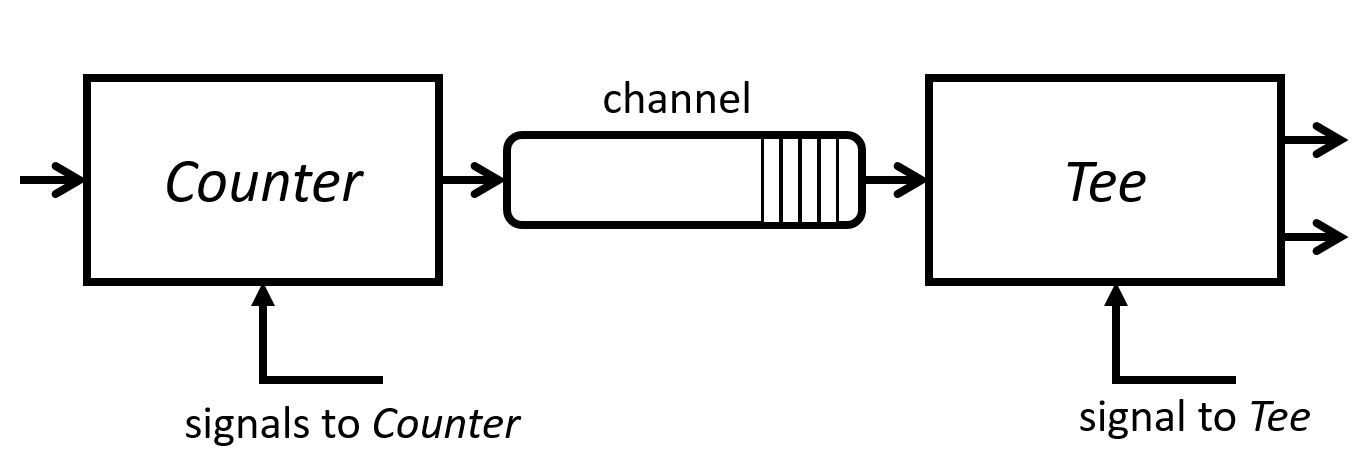
\includegraphics[width=4in]{channel}
\caption{连接两个元件的通道} \label{fig:channel}
\end{figure}

每次通道读写操作的基本单位为帧,每个帧的大小固定为64字节,其中头部包含元数据,
数据载荷长32字节。其结构及成员定义如图~\ref{fig:flit}、代码~\ref{code:flitdef} 所示。
\begin{figure}[htbp]
\centering
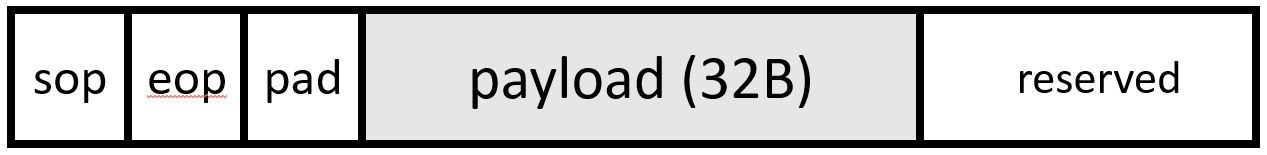
\includegraphics[width=4in]{flit}
\caption{帧结构} \label{fig:flit}
\end{figure}

\lstinputlisting[caption=帧成员定义, label=code:flitdef]{code/flit.cl}

以完整包为代表的大段数据会被拆分为多个帧在元件之间传播。
其中第一帧的包开始位(start of packet, \lstinline$sop$)置为真,
最后一帧的包结束位(end of packet, \lstinline$eop$)置为真。
如果数据载荷小于32字节,那么最后一帧的留白(padding, \lstinline$pad$)域指代载荷的尾部留白区段大小。
将大的包拆分为帧,不仅能够降低延迟,还有助于提升处理包数据的各级流水线之间并行化程度。

在定义完各个元件之后,通过ClickNP配置文件将元件连接为有向图,使其互连,形成总的计算系统,
代码~\ref{code:cfg} 为一个远程直接内存访问(remote direct memory access, RDMA)处理器的配置文件,
其开头部分描述该系统依赖的元件类型,随后将元件实例化,并用箭头表示其通道连接关系,
自左侧元件的输出端口指向右侧元件的输入端口,方括号中的数字代表端口号。
\begin{figure}[htbp]
\centering
\lstinputlisting[caption=ClickNP配置文件示例, label=code:cfg]{code/sample.cfg}
\note{\lstinline$host$关键字代表将\lstinline$Count$元件实例化为主机工作线程,
@表示该元件接收主机发来的信号。\lstinline$from_tor$和\lstinline$to_tor$分别为FPGA网卡的输出和输入端口。}
\end{figure}

\subsection{编程语言}
ClickNP元件类似于面向对象语言中的对象,可以用C++这样的语言定义。
但现有的很多高级编程工具只支持C语言,而将高级语言转化为C语言的工作是乏味的,
因此我们采用的是针对定义元件的需要对C语言进行扩展这种途径。

\begin{figure}[htbp]
\centering
\lstinputlisting[caption=包计数器元件定义, label=code:count]{code/Count.cl}
\end{figure}
代码~\ref{code:count} 是一个包计数器元件的定义。\lstinline$.element$关键字定义元件名称;
尖括号内为输入输出端口数;\lstinline$.state$关键字定义本地状态\lstinline$count$计数器;
\lstinline$.init$关键字定义初始化函数,将\lstinline$count$的初值置零;
\lstinline$.handler$关键字定义处理函数,每当收到帧的\lstinline$sop$域为真时将计数器加一;
\lstinline$.signal$关键字定义信号函数,每当收到主机发来的任意信号帧时,
将当前包计数作为信号载荷发给主机。

ClickNP内建了一系列与端口进行数据交互的函数接口,如表~\ref{tab:operations} 所示。
\begin{table}[htbp]
\centering
\caption{ClickNP内建接口} \label{tab:operations}
\begin{tabular}{l|l}
\hline
\lstinline$uchar get_input_port()$         & 获取第一个有帧输入的端口号 \\
\hline
\lstinline$bool test_input_port(uchar id)$ & 检查\lstinline$id$号端口有无帧输入 \\
\hline
\lstinline$flit read_input_port(uchar id)$ & 自\lstinline$id$号端口读取帧 \\
\hline
\lstinline$flit peek_input_port(uchar id)$ & 窥视\lstinline$id$号输入端口的帧 \\
\hline
\lstinline$void set_output_port(uchar id,$ & 向\lstinline$id$号端口写入帧, \\
\lstinline$flit x)$                        & 在处理函数执行到返回时, \\
                                           & 该帧将被写入通道 \\
\hline
\lstinline$ClSignal read_signal()$         & 自信号输入端口读取帧 \\
\hline
\lstinline$void set_signal(ClSignal p)$    & 向信号输出端口写入帧 \\
\hline
\end{tabular}
\end{table}

\subsection{编译工具链}
ClickNP工具链以ClickNP编译器为前端,以Visual Studio、GCC等C/C++编译器、
Altera OpenCL SDK、Xilinx Vidado HLS等高级编程工具为后端。
开发人员需要完成三部分工作:
\begin{enumerate}
\item 定义元件,每个元件实现一小部分简单的功能;
\item 编写配置文件,描述元件之间的连接关系,以组成完整的逻辑系统;
\item 设计主机管理进程,初始化各元件并在运行时根据用户输入控制元件行为。
\end{enumerate}

以上三部分源程序由ClickNP编译器翻译为主机程序和FPGA程序两部分中间代码。
前者可由普通的C/C++编译器编译为目标文件,
后者需要由商业化高级编程工具合成为FPGA目标文件。

\chapter{RoCEv2的ClickNP实现}
\section{对RoCEv2协议进行抓包分析}
为了充分了解RoCEv2协议,我们利用微软亚洲研究院程鹏研究员基于NetDirect开发的ndping、ndrping工具发送RoCEv2包,
并使用IbDump工具对其进行抓包分析。

我们的实验在与同一交换机相连的两台之间进行,期间基本不存在丢包的情况,
所以初期我们只能抓到无丢包情况下的包。

为了解决这一问题,我基于ClickNP平台开发了丢包器,能够在用户的控制下,以一定的概率丢包。
将丢包逻辑写入FPGA,将主机与交换机之间用FPGA串联,即可在FPGA上将包拦截下来。

将丢包率调整为10\%左右时,可以较好地观察到丢包与重传时所发的包。

在抓包的过程中,我们发现一些根据协议本应出现的包没有被观察到,
并据此猜测IbDump没有将流经网卡的包全部记录下来。

为了验证这一猜测,我们改在FPGA上抓包。在丢包器的下游增设抓包器,在记录包的同时将其发出。

在使用FPGA抓包的过程中,我们发现当发包频率加快时,会出现阻塞情况。
这是因为抓包器将包记录在主机上需要通过PCIe接口发送数据,
而PCIe接口的数据带宽低于FPGA网卡的带宽,因此缓冲区会被迅速写满,随后不再响应网卡的输入请求。

为了解决这一问题,我对ndping、ndrping的代码进行了修改,将原有的连续发送RDMA请求改为有时间间隔地发送RDMA请求。
虽然在请求长度较大时仍然会出现阻塞情况,但因为我们在FPGA上的抓包实验侧重于对丢包情况进行分析,
因此不需要发送长度太大的RDMA请求。

实验表明,FPGA的抓包结果中确实出现了之前IbDump没有记录下来的包,
这证实了我们的猜测,也验证了我们对于RoCEv2协议的初步理解。

在IbDump与FPGA两个抓包工具获取到的日志基础上进行分析,使我们加深了对RoCEv2协议的认识。

\begin{figure}[htbp]
\centering
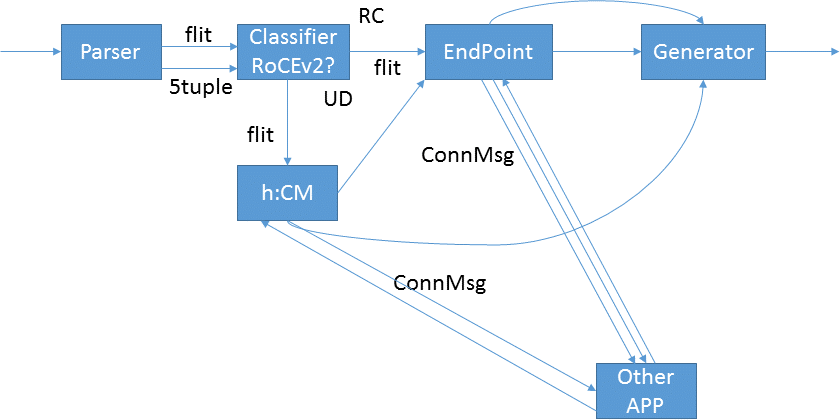
\includegraphics[width=4in]{roce}
\caption{RoCEv2各元件及其连接关系} \label{fig:roce}
\end{figure}

\begin{figure}[htbp]
\centering
\lstinputlisting[caption=RoCEv2项目的ClickNP配置文件, label=code:rocecfg]{code/RoCE.cfg}
\end{figure}
\section{项目实现}
\subsection{总体设计}
RoCEv2项目包含如下元件:
\begin{description}
\item[RoCE\_Classifier包分类器]将收到的包进行分类,将连接相关请求转发至连接管理器,将数据请求转发至适配器。
\item[RoCE\_Connector连接管理器]根据连接请求,建立、维护、断开连接。
\item[应用程序]向适配器发起应用RDMA请求。
\item[RoCE\_Endpoint适配器]与应用程序交互,将用户的请求转发至包生成器,并向应用程序发送反馈。
\item[RoCE\_Gen包生成器]将连接管理器和适配器发来的请求翻译为网络协议包。
\end{description}

图~\ref{fig:roce} 展示各元件间的连接关系,其配置文件如代码~\ref{code:rocecfg} 所示。

\subsection{包生成器设计}
我设计的包生成器有2个输入端口和1个输出端口。
其中输入端口1与适配器相连,输入端口2与连接管理器相连;输出端口与网卡相连。

当输入端口有收到发包请求时,包生成器根据收到的元数据填写待发送帧的各个域,
并维护其操作码及序列号两个状态,每周期处理一帧,直到最后一帧发送完毕,读取下一个请求。

值得一提的是,由于元数据帧的信息密度大于要发送的帧,
所以只要输入端有源源不断的发包请求,输出端就不会忙等,
不需要手工维护多级流水线及其缓冲区即可充分利用设备的吞吐率。

包生成器的大致框架如代码~\ref{code:rocegen} 所示。
\lstinputlisting[caption=RoCE\_Gen包生成器示意,label=code:rocegen]{code/RoCE_Gen.cl}
截至我从微软亚洲研究院离职时,包生成器已实现CM ConnectionReply、CM ReadyToUse、
Acknowledge、RC RDMA Read Request等功能,代码量不足八百行,
预计实现全部功能只需要四千行代码。

另外,看似比较大的代码量不代表程序效率低下。因为同一个分支内不存在数据依赖,
所以这些代码在FPGA中很容易实现并行化,可以认为是同时执行。

\chapter{性能测试}

\chapter{结论}
本文利用FPGA平台对网络协议功能进行加速。
我们注意到ClickNP平台可以用类似于软件开发的方式设计FPGA上的网络功能,
且可以实现CPU与FPGA之间的协作,获得性能提升。

评测结果表明,相比于前沿的软件网络应用,ClickNP可以将吞吐率提升一个数量级,
同时将延迟降低一个数量级。这充分说明FPGA能够有效提升数据中心网络的性能。


\bibliography{bib/tex}

\appendix
%\chapter{论文规范}

%\backmatter
%\input{chapters/publications}

\end{document}
